\section{Max-flow: Disposition}
\begin{enumerate}
	\item Flow network
	\begin{itemize}
		\item Source/Sink
		\item Capacity
		\item Supersource/supersink.
	\end{itemize}
	\item Flow $|f|$
	\begin{itemize}
		\item Capacity Constraint: $\forall u,v\in V: 0 \leq f(u,v) \leq c(u,v)$
		\item Flow conservation: $\forall u\in V - \{s,t\}:
			\sum_{v\in V} f(u,v) = \sum_{v\in V} f(v,u)$
	\end{itemize}
	\item Ford-Fulkerson
	\begin{itemize}
		\item Residual network
		\item Augmenting paths
		\item Cuts
	\end{itemize}
\end{enumerate}
\section{Max-flow: Notes}
%%
A flow network $G = (V,E)$ is a directed graph where each edge $(u,v) \in E$ has
a non-negative capacity $c(u,v) \geq 0$. If there is an edge $(u,v) \in E$ then
there is no edge $(v,u) \in E$. If $(u,v) \notin E$ then $c(u,v) = 0$ for convenience.
When $(u,v) \notin E$, $f(u,v) = 0$.

Flow networks have a source $s$ and a sink $t$. For each vertex $v \in V$, the flow
network contains a path $s \leadsto v \leadsto t$. The graph is therefore connected, meaning
$|E| \geq |V| - 1$.

A flow is a real-valued function $f : V \times V \rightarrow \mathbb{R}$ that satisfies
two properties:
%%
\begin{description}
	\item[Capacity constraint:] For all $u,v \in V$, $0 \leq f(u,v) \leq c(u,v)$

	\item[Flow conservation:] For all $u \in V - \{s,t\}$, 
	$\sum_{v \in V} f(u,v) = \sum_{v \in V} f(v,u)$.
\end{description}
%%
The value of a flow, $|f|$, is defined as:
%%
\begin{align*}
	|f| = \sum_{v \in V} f(s,v) - \sum_{v \in V} f(v,s)
\end{align*}
%%
In the \textbf{maximum-flow} problem, we are given a flow network $G$ and we wish to find
a maximum flow.

Edges are anti-parallel if there is both an edge $(u,v)$ and an edge $(v,u)$. This is not allowed,
and to get around this we instead introduce a new edge $x$ and re-structure the edges as follows:
$(u,x), (x,v), (v,u)$. The capacity of the new edges involving $x$ is the same as the capacity from
$(u,v)$. See page 711 in the book for an example.

\subsection{Multiple sources and sinks}
%%
This can be accounted for by introducing a \textbf{supersink} and \textbf{supersource} with infinite
flow and capacity out to all of the sources and from all of the sinks to the supersink. See page 713.

\subsection{Ford-Fulkerson}
%%
Three basic principles: \textbf{residual networks}, \textbf{augmenting paths} and \textbf{cuts}.
Essential for \textbf{max-flow min-cut} theorem (Theorem 26.6).

Intuition is as follows: We have a flow network $G$. We iteratively alter the flow of $G$, 
by finding an augmenting path in an associated residual network $G_f$. Once we know the edges
that belong to an augmenting path, we can identify specific edges in $G$ to increase or decrease
the flow of. Each iteration increases overall flow, but it may do so by decreasing the flow along
certain edges. This is repeated until the residual network $G_f$ has no more augmenting paths.

\textbf{max-flow min-cut} shows that upon termination, this yields a maximum flow.

\subsubsection{Residual network}
\begin{figure}
	\centering
	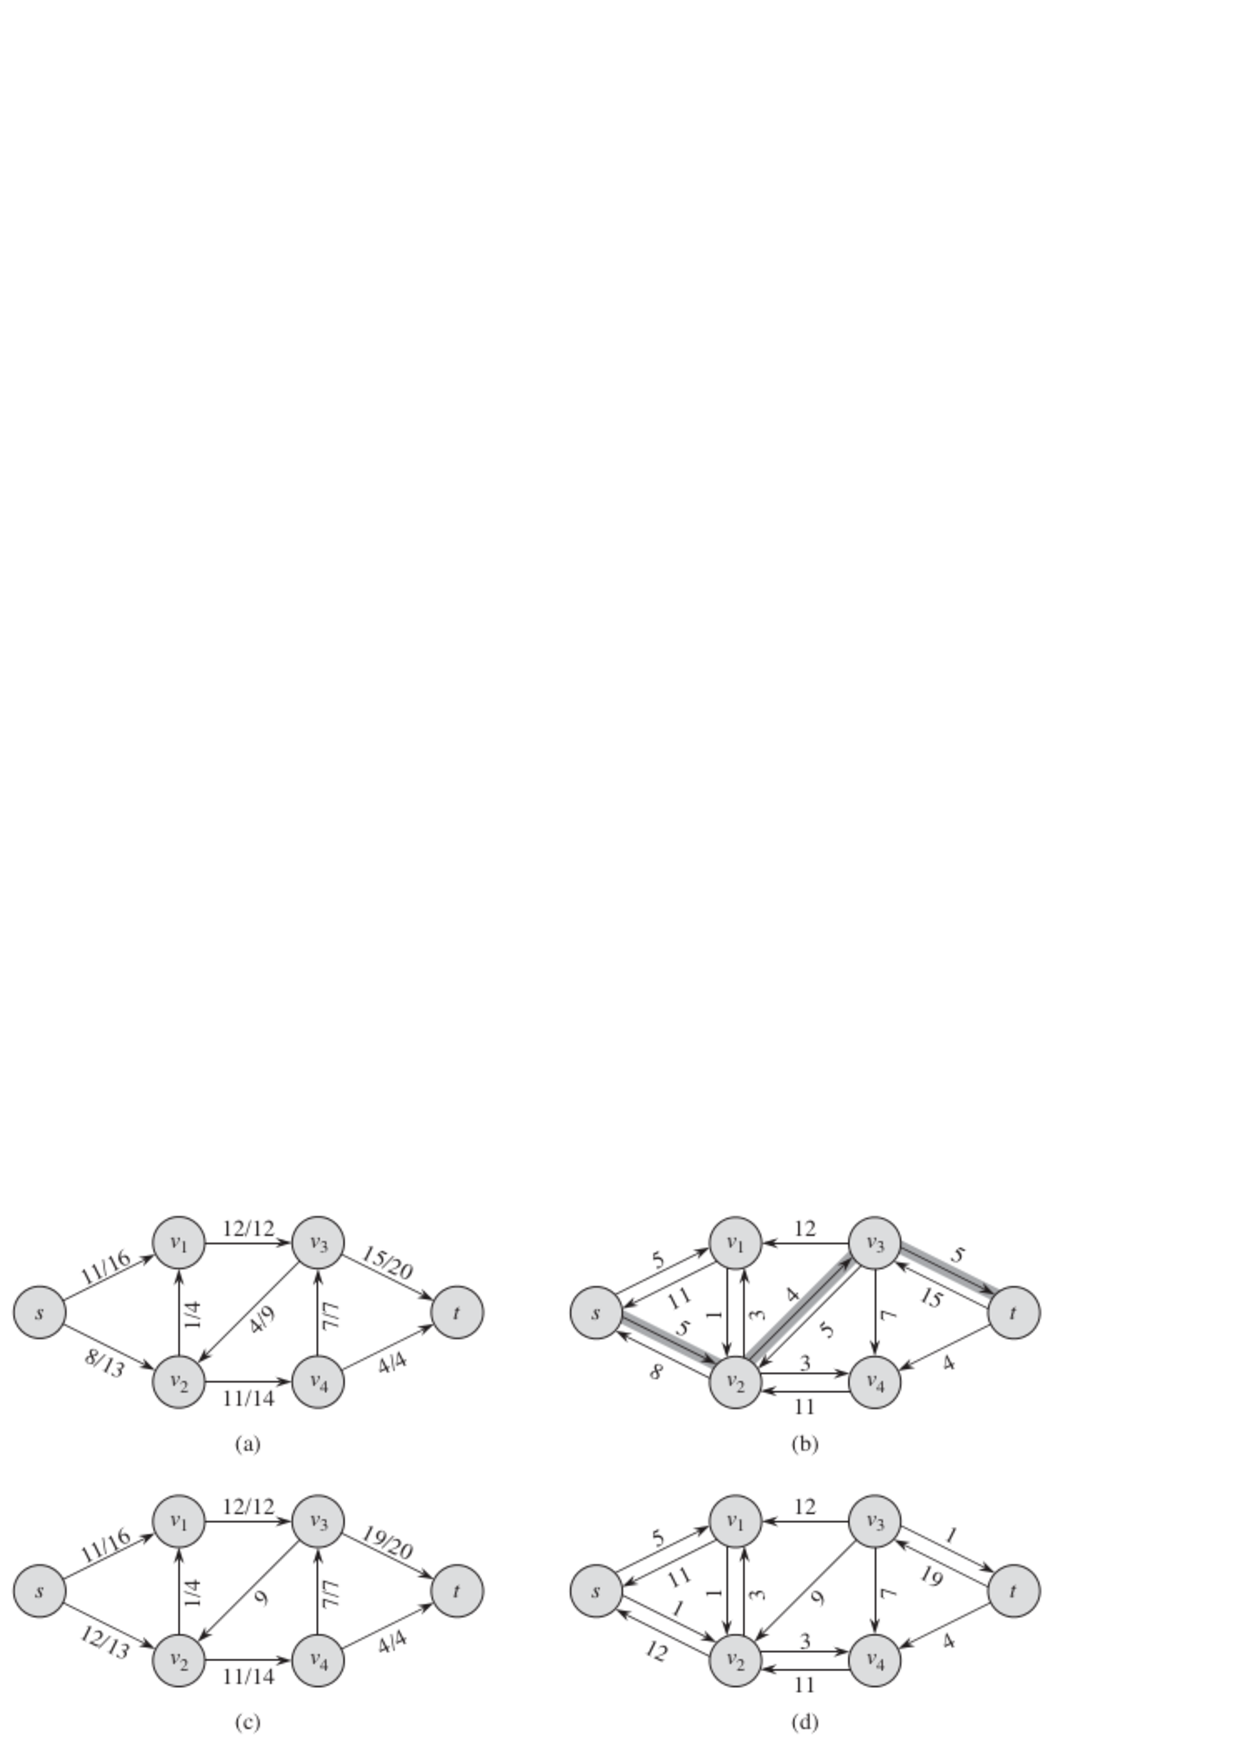
\includegraphics[width=\textwidth]{images/augmenting_paths}
\end{figure}
%%
Given a network $G = (V,E)$ with a flow $f$, the \textbf{residual network}
of $G$ induced by $f$ is $G_f = (V, E_f)$, where
%%
\[
	E_f = \{(u,v) \in V \times V : c_f(u,v) > 0\}.
\]
%%
Residual capacity $c_f(u,v)$ is defined by
%%
\[
 c_f(u,v) =
  \begin{cases}
  	c(u,v) - f(u,v) & \text{if } (u,v) \in E, \\
  	f(v,u) & \text{if } (v,u) \in E, \\
  	0 & \text{otherwise}
  \end{cases}
\]
%%
\textit{Note:} that $(u,v) \in E$ implies $(v,u) \notin E$, so there is always only one of the three
above cases that applies. 

Because the edges in $E_f$ are either edges from $E$ or an edge in the opposite direction,
$|E_f| \leq 2|E|$.

Intuition: A residual network $G_f$ consists of edges with capacities that
represent how we can alter the flow on edges of $G$. $G$ can admit an
additional amount of flow along an edge, equal to the capacity minus the
current flow. If the edge can admit more flow, that edge is placed into $G_f$
with a value of $c_f(u,v) = c(u,v) - f(u,v)$. The residual network may also
contain edges that are not in $G$: In order to represent a possible decrease
of a flow $f(u,v)$ on an edge in $G$, we place an edge $(v,u)$ into $G_f$ with
residual capacity $c_f(v,u) = f(u,v)$. In other words, an edge that can admit
flow in the opposite direction, at most cancelling out flow entirely. See
Figure~\ref{fig:aug_paths} for an example.

Flows in a residual network satisfy the definition of a flow, but with respect to capacities
$c_f$ in the network $G_f$. If $f$ is a flow in $G$ and $f'$ is a flow in the corresponding residual
network $G_f$, we define $f \uparrow f'$, the \textbf{augmentation flow} of f by f', as a function
from $V \times V$ to $\mathbb{R}$ defined by
%%
\[
  (f \uparrow f')(u,v) =
  \begin{cases}
  	f(u,v) + f'(u,v) - f'(v,u) & \text{if } (u,v) \in E, \\
  	0 & \text{otherwise.}
  \end{cases}
\]

Intuition: Increase the flow ($f(u,v)$) by $f'(u,v)$, but decrease it by the flow in the
opposite direction ($f'(v,u)$). Pushing flow in the reverse direction is also called \textbf{cancellation}.

\subsubsection{Augmenting path}
An augmenting path $p$ is a simple path from $s$ to $t$ in the residual network $G_f$. By the definition
of a residual network, we may increase the flow of an edge $(u,v)$ by up to $c_f(u,v)$ without violating the
capacity constraint on whichever of $(u,v)$ and $(v,u)$ is in the original flow network $G$.

The maximum amount by which we can increase flow on each edge of an augmenting path $p$ is the
\textbf{residual capacity} of $p$, given by $c_f(p) = min\{c_f(u,v) : (u,v) \text{ is on p}\}$. More specifically,
if $p$ is an augmenting path in $G_f$, we define a function $f_p : V \times V \rightarrow \mathbb{R}$ as
%%%
\[
	f_p(u,v) =
	\begin{cases}
		c_f(p) & \text{if } (u,v) \text{is on } p, \\
		0 & \text{otherwise}.
	\end{cases}
\]
%%
Then $f_p$ is a flow in $G_f$ with value $|f_p| = c_f(p) > 0$. See Lemma 26.2, page 720. It remains to be
shown that augmenting $f$ by $f_p$ produces a different flow in $G$ whose value is closer to the maximum.
Corollary 26.3 on page 720 shows this by immediate proof, using Lemma 26.1 and 26.2.

\subsubsection{Cuts of a network}
We know, based on the above, that we can augment flows in $G$ and that doing
so can produce a new flow closer to the maximum. But how do we know that when
it terminates, the algorithm has in fact found a maximum flow? Max-flow min-
cut tells us that a flow is maximum only if its residual network contains no
augmenting paths.

A \textbf{cut} $(S,T)$ of a flow network $G = (V,E)$ is a partition of $V$ into $S$ and $T=V-S$ such that
$s \in S$ and $t \in T$. If $f$ is a flow then the \textbf{net flow} $f(S,T)$ across the cut $(S,T)$ is
defined to be
%
\[
	f(S,T) = \sum_{u \in S} \sum_{v \in T} f(u,v) - \sum_{u in \S} \sum_{v \in T} f(v,u)
\]
%
The \textbf{capacity} of the cut $(S,T)$ is
%
\[
	c(S,T) = \sum_{u \in S} \sum_{v \in T} c(u,v)
\]
%
Intuitively, the capacity of the cut is the capacity of all vertices going
from $S$ to $T$, while the flow is the flow of vertices going from $S$ to $T$,
minus the flow going from $T$ to $S$. A \textbf{minimum cut} of a network is a
cut whose capacity is minimum over all cuts of the network.

Theorem 26.6 (Max-flow min-cut theorem, p. 723/724) involves proving the equivalence of 3
different conditions:
\begin{enumerate}
	\item $f$ is a maximum flow of $G$. \label{max-min-theorem:1}
	\item The residual network $G_f$ contains no augmenting paths. \label{max-min-theorem:2}
	\item $|f| = c(S,T)$ for some cut $(S,T)$ of $G$. \label{max-min-theorem:3}
\end{enumerate}

\ref{max-min-theorem:1} => \ref{max-min-theorem:2}:
%
Assume that $f$ were a maximum flow in $G$ and there \textbf{was} an augmenting path. This
means, by the proof of augmenting paths, that we could create a new flow $f'$ in $G$ with a strictly
larger flow value than $f$, i.e. that $|f'| > |f|$. This contradicts $f$ being a maximum flow.

\ref{max-min-theorem:2} => \ref{max-min-theorem:3}:
%
Suppose that there are no augmenting paths, that is there is no path from $s$ to $t$ in $G_f$.

Define $S = \{v\in V: \text{there exists a path from $s$ to $v$ in $G_f$}\}$. That is, the set $S$
contains all those vertices for which there could be pushed more flow along, but which perhaps have
not because a later capacity limits that possibility. Define $T = V-S$. A partition $(S,T)$ is a cut,
where $s\in S$ and $t \notin S$ (since there is no path from $s$ to $t$, or we would not have a maximum
flow).

Consider two vertices $(u,v)$ where $u\in S$ and $v\in T$:

If $(u,v)\in E$, we must have that $f(u,v) = c(u,v)$. If this were not the case we would have 
$(u,v)\in E_f$, since we would be able to push more flow out until at capacity. Then, by the definition 
of $S$ we would have that $v\in S$. This is a contradiction.

If $(v,u)\in E$, we must have that $f(v,u) = 0$. If this were not the case we would have
$(v,u)\in E_f$, since the residual capacity $c_f(u,v) = f(v,u)$ would be positive. This
means $(u,v)\in E_f$, and we would have that $v\in S$. This is a contradiction.

